\input{../header}
\usepackage{pgfplots}
\rhead{Your name: \rule{8cm}{0.15mm}}

\begin{document}
%


%\onehalfspacing
\allowdisplaybreaks
%##################################################################
\section{Learning targets DF1 and DFa, version 2}

Arapaho Glacier is a mountain glacier in Roosevelt National Forest,
west of Boulder, CO. The following table\footnote{
Haugen, B., Scambos, T., Pfeffer, T., \& Anderson, R. (2010). Twentieth-century changes in the thickness and extent of Arapaho Glacier, Front Range, Colorado. \textit{Arctic, Antarctic, and Alpine Research, 42}(2), 198-209.}
gives the surface area, $A(t)$, in square meters, of Arapaho Glacier in the year $t$. 
\begin{center}
	\begin{tabular}{|c|c|c|c|c|}
	\hline
	$t$ & 1900 & 1960 & 1973 & 1999\\
	\hline
	$A(t)$ & 338,282 & 250,764 & 225,000 & 162,027\\
	\hline
	\end{tabular}
 \end{center}
	
\begin{enumerate}[leftmargin=0pt]

\item Compute an approximation for $A'(1960)$, and {\bf include units} for this number.\\
Write a sentence explaining what the number means about how the area of the glacier is changing.\\
\textbf{Don't say ``per,'' and don't say ``rate of change''}. 

\vfill
\vfill

\item Compute an approximation for $A'(1999)$, and {\bf include units} for this number.\\
Do you think your approximation is too high or too low? Why?

\vfill
\vfill

\item How does $A'(1960)$ compare to $A'(1999)$? Is that good or bad?
\vfill
\end{enumerate}

%%%%%%%%%%%%%%%%%%%%%%%%%%%%%%%%%%%%%%%%%%%%%%%%%%%%%%%%%
\pagebreak
%%%%%%%%%%%%%%%%%%%%%%%%%%%%%%%%%%%%%%%%%%%%%%%%%%%%%%%%%

\section{Learning target DF2, version 2}

Suppose that  \(g(w) = 6 \, w^{3} - 2 \, w^{2} - 9 \, w - 2\). Use the limit definition of the derivative to find $g'(w)$.

\vspace{1em} 

Algebra hint: $(w+h)^3 = w^3 + 3w^2 h + 3w h^2 + h^3$.

%%%%%%%%%%%%%%%%%%%%%%%%%%%%%%%%%%%%%%%%%%%%%%%%%%%%%%%%%
\pagebreak
%%%%%%%%%%%%%%%%%%%%%%%%%%%%%%%%%%%%%%%%%%%%%%%%%%%%%%%%%

\section{Learning target DFb, version 2}

Here is the graph of some wacky function $h(t)$:

\begin{center}
    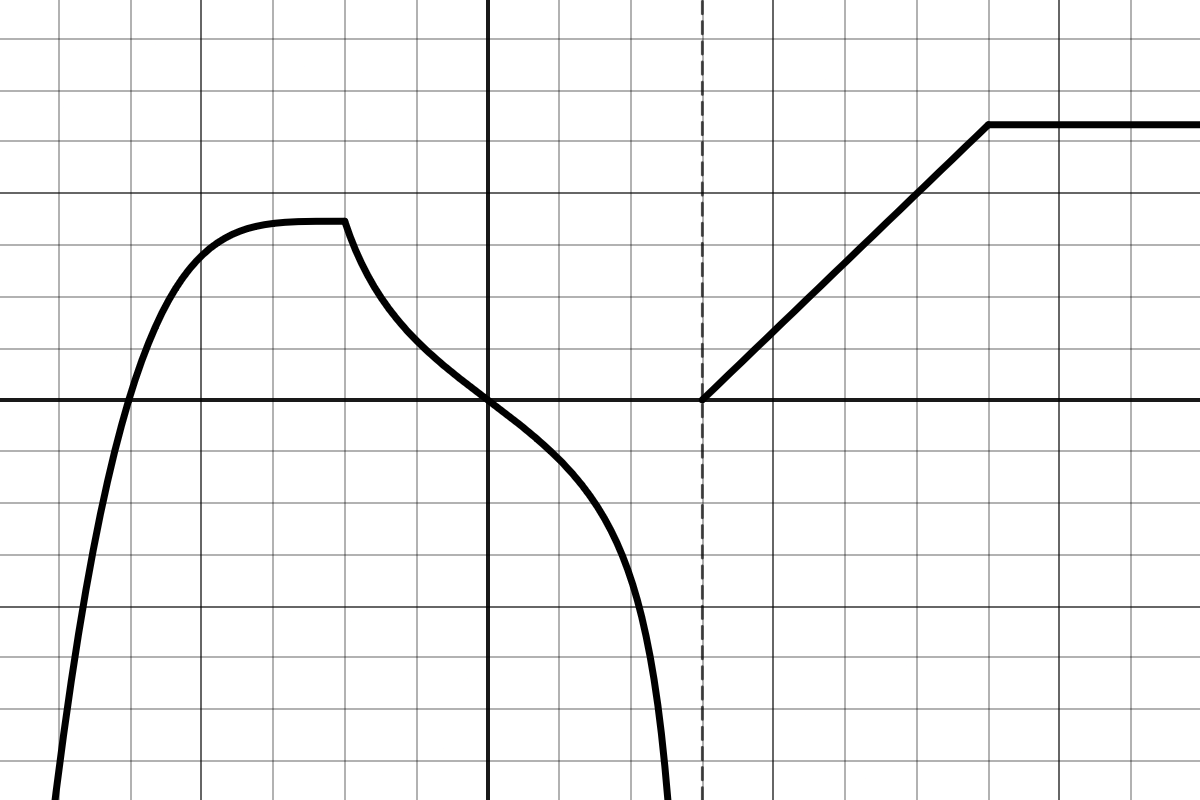
\includegraphics[width=0.9\textwidth]{../images/DFb-v2.png}    
\end{center}


Sketch the graph of $h'(t)$ on the blank axes below.

\begin{center}
    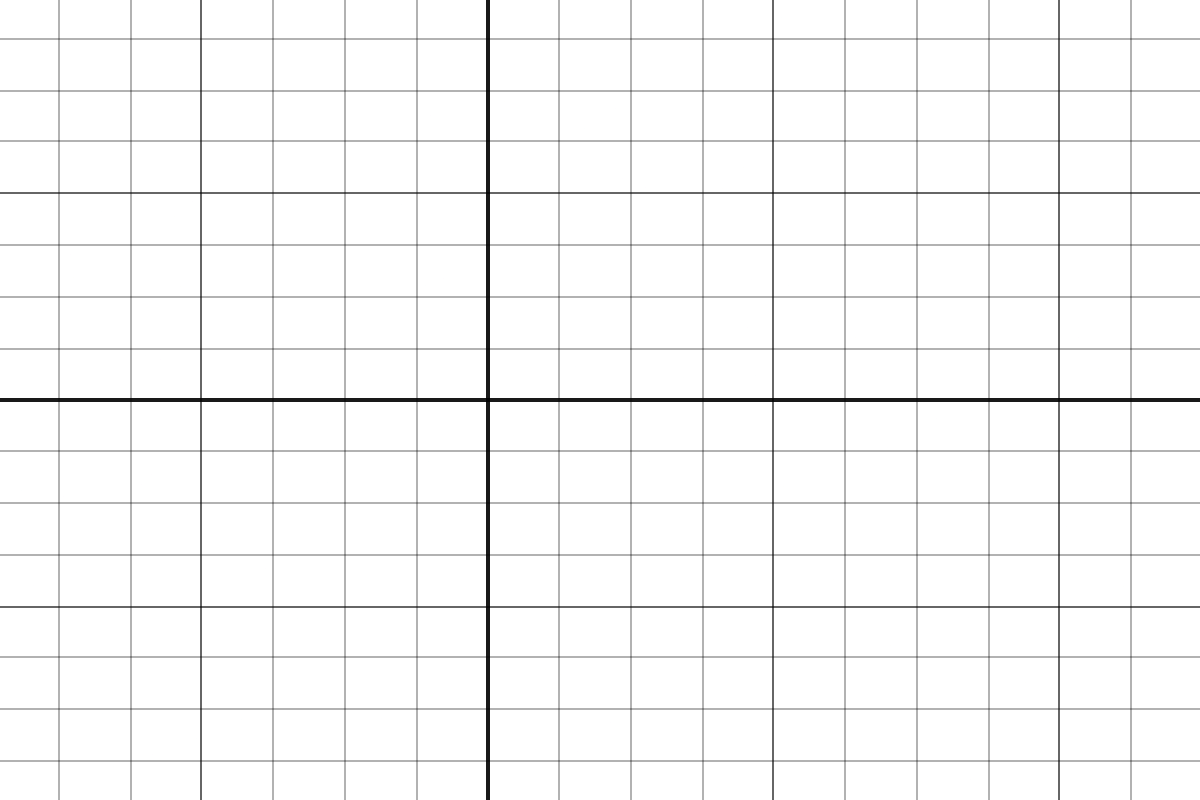
\includegraphics[width=0.9\textwidth]{../images/DFb-v2-blank.png}    
\end{center}

\end{document}